%%%%%%%%%%%%%%%%%%%%%%%%%%%%%%%%%%%%%%%%%
% Beamer Presentation
% LaTeX Template
% Version 2.0 (March 8, 2022)
%
% This template originates from:
% https://www.LaTeXTemplates.com
%
% Author:
% Vel (vel@latextemplates.com)
%
% License:
% CC BY-NC-SA 4.0 (https://creativecommons.org/licenses/by-nc-sa/4.0/)
%
%%%%%%%%%%%%%%%%%%%%%%%%%%%%%%%%%%%%%%%%%

%----------------------------------------------------------------------------------------
%	PACKAGES AND OTHER DOCUMENT CONFIGURATIONS
%----------------------------------------------------------------------------------------

\documentclass[
	11pt, % Set the default font size, options include: 8pt, 9pt, 10pt, 11pt, 12pt, 14pt, 17pt, 20pt
	%t, % Uncomment to vertically align all slide content to the top of the slide, rather than the default centered
	%aspectratio=169, % Uncomment to set the aspect ratio to a 16:9 ratio which matches the aspect ratio of 1080p and 4K screens and projectors
	hmargin=1cm,vmargin=0cm,head=0.5cm,headsep=0pt,foot=0.5cm,margin=2cm
]{beamer}

% Hide navigation symbols
\setbeamertemplate{navigation symbols}{}

\usepackage{caption}
\captionsetup[figure]{labelsep=space}
\renewcommand{\figurename}{}
\renewcommand{\tablename}{}
\graphicspath{{images/}{./}} % Specifies where to look for included images (trailing slash required)
% \usepackage{minted}
\usepackage{amsmath}
\usepackage{multirow}
\usepackage{color, colortbl}
\usepackage{xcolor}
\usepackage{booktabs} % Allows the use of \toprule, \midrule and \bottomrule for better rules in tables
\usepackage{graphicx}
\usepackage{minibox}
\renewcommand{\arraystretch}{1.1} % Default value: 1
\definecolor{darkGreen}{RGB}{9,150,3} 
% \usepackage[margin=2cm]{geometry}
% \usepackage[most]{tcolorbox}
% \newtcolorbox{mytextbox}[1][]{%
%   sharp corners,
%   enhanced,
%   colback=white,
%   height=10cm,
%   attach title to upper,
%   #1
% }
%----------------------------------------------------------------------------------------
%	SELECT LAYOUT THEME
%----------------------------------------------------------------------------------------
%
% Beamer comes with a number of default layout themes which change the colors and layouts of slides. Below is a list of all themes available, uncomment each in turn to see what they look like.

%\usetheme{default}
%\usetheme{AnnArbor}
%\usetheme{Antibes}
%\usetheme{Bergen}
%\usetheme{Berkeley}
% \usetheme{Berlin}
%\usetheme{Boadilla}
% \usetheme{CambridgeUS}
% \usetheme{Copenhagen}
% \usetheme{Darmstadt}
% \usetheme{Dresden}
% \usetheme{Frankfurt}
% \usetheme{Goettingen}
% \usetheme{Hannover}
% \usetheme{Ilmenau}
% \usetheme{JuanLesPins}
% \usetheme{Luebeck}
\usetheme{Madrid}
%\usetheme{Malmoe}
%\usetheme{Marburg}
%\usetheme{Montpellier}
%\usetheme{PaloAlto}
%\usetheme{Pittsburgh}
%\usetheme{Rochester}
%\usetheme{Singapore}
%\usetheme{Szeged}
%\usetheme{Warsaw}

%----------------------------------------------------------------------------------------
%	SELECT COLOR THEME
%----------------------------------------------------------------------------------------

% Beamer comes with a number of color themes that can be applied to any layout theme to change its colors. Uncomment each of these in turn to see how they change the colors of your selected layout theme.

% \usecolortheme{albatross}
% \usecolortheme{beaver}
% \usecolortheme{beetle}
% \usecolortheme{crane}
% \usecolortheme{dolphin}
% \usecolortheme{dove}
% \usecolortheme{fly}
% \usecolortheme{lily}
% \usecolortheme{monarca}
% \usecolortheme{seagull}
% \usecolortheme{seahorse}
\usecolortheme{spruce}
% \usecolortheme{whale}
% \usecolortheme{wolverine}

%----------------------------------------------------------------------------------------
%	SELECT FONT THEME & FONTS
%----------------------------------------------------------------------------------------

% Beamer comes with several font themes to easily change the fonts used in various parts of the presentation. Review the comments beside each one to decide if you would like to use it. Note that additional options can be specified for several of these font themes, consult the beamer documentation for more information.

\usefonttheme{default} % Typeset using the default sans serif font
%\usefonttheme{serif} % Typeset using the default serif font (make sure a sans font isn't being set as the default font if you use this option!)
\usefonttheme{structurebold} % Typeset important structure text (titles, headlines, footlines, sidebar, etc) in bold
%\usefonttheme{structureitalicserif} % Typeset important structure text (titles, headlines, footlines, sidebar, etc) in italic serif
%\usefonttheme{structuresmallcapsserif} % Typeset important structure text (titles, headlines, footlines, sidebar, etc) in small caps serif

%------------------------------------------------

%\usepackage{mathptmx} % Use the Times font for serif text
\usepackage{palatino} % Use the Palatino font for serif text

%\usepackage{helvet} % Use the Helvetica font for sans serif text
\usepackage[default]{opensans} % Use the Open Sans font for sans serif text
%\usepackage[default]{FiraSans} % Use the Fira Sans font for sans serif text
%\usepackage[default]{lato} % Use the Lato font for sans serif text

%----------------------------------------------------------------------------------------
%	SELECT INNER THEME
%----------------------------------------------------------------------------------------

% Inner themes change the styling of internal slide elements, for example: bullet points, blocks, bibliography entries, title pages, theorems, etc. Uncomment each theme in turn to see what changes it makes to your presentation.

%\useinnertheme{default}
\useinnertheme{circles}
% \useinnertheme{rectangles}
% \useinnertheme{rounded}
%\useinnertheme{inmargin}

%----------------------------------------------------------------------------------------
%	SELECT OUTER THEME
%----------------------------------------------------------------------------------------

% Outer themes change the overall layout of slides, such as: header and footer lines, sidebars and slide titles. Uncomment each theme in turn to see what changes it makes to your presentation.

% \useoutertheme{default}
% \useoutertheme{infolines}
\useoutertheme{miniframes}
% \useoutertheme{smoothbars}
% \useoutertheme{sidebar}
%\useoutertheme{split}
% \useoutertheme{shadow}
% \useoutertheme{tree}
%\useoutertheme{smoothtree}

%\setbeamertemplate{footline} % Uncomment this line to remove the footer line in all slides
%\setbeamertemplate{footline}[page number] % Uncomment this line to replace the footer line in all slides with a simple slide count

%\setbeamertemplate{navigation symbols}{} % Uncomment this line to remove the navigation symbols from the bottom of all slides

%----------------------------------------------------------------------------------------
%	PRESENTATION INFORMATION
%----------------------------------------------------------------------------------------

\title[LAB 02: Intro to MIPS Assembly]{LAB 02: Introduction to MIPS Assembly Programing} % The short title in the optional parameter appears at the bottom of every slide, the full title in the main parameter is only on the title page

% \subtitle{Optional Subtitle} % Presentation subtitle, remove this command if a subtitle isn't required

\author[S. AlSaleh]{Saleh AlSaleh \\ \smallskip \textit{salehs@kfupm.edu.sa}} % Presenter name(s), the optional parameter can contain a shortened version to appear on the bottom of every slide, while the main parameter will appear on the title slide

\institute[KFUPM]{King Fahd University of Petroleum and Minerals \\ College of Computing and Mathematics \\ Computer Engineering Department} % Your institution, the optional parameter can be used for the institution shorthand and will appear on the bottom of every slide after author names, while the required parameter is used on the title slide and can include your email address or additional information on separate lines

\date[January 22, 2023]{COE301: Computer Architecture \\ Term 222} % Presentation date or conference/meeting name, the optional parameter can contain a shortened version to appear on the bottom of every slide, while the required parameter value is output to the title slide

%----------------------------------------------------------------------------------------

\begin{document}

%----------------------------------------------------------------------------------------
%	TITLE SLIDE
%----------------------------------------------------------------------------------------

\begin{frame}
	% Output the title slide, automatically created using the text entered in the PRESENTATION INFORMATION block above
	\titlepage
\end{frame}

%----------------------------------------------------------------------------------------
%	TABLE OF CONTENTS SLIDE
%----------------------------------------------------------------------------------------

% The table of contents outputs the sections and subsections that appear in your presentation, specified with the standard \section and \subsection commands. You may either display all sections and subsections on one slide with \tableofcontents, or display each section at a time on subsequent slides with \tableofcontents[pausesections]. The latter is useful if you want to step through each section and mention what you will discuss.

\begin{frame}
	\frametitle{Agenda} % Slide title, remove this command for no title
	
	\tableofcontents % Output the table of contents (all sections on one slide)
	% \tableofcontents[pausesections] % Output the table of contents (break sections up across separate slides)
\end{frame}

%----------------------------------------------------------------------------------------
%	PRESENTATION BODY SLIDES
%----------------------------------------------------------------------------------------

\section{Prev. Side Project} 
\begin{frame}
	\frametitle{Previous Side Project: AES Overview}
	
	\begin{itemize}
		\item Advanced Encryption Standard (AES) or Rijndael developed by Vincent Rijmen and Joan Daemesn is a symmetric key encryption and decryption algorithm.
		\item It was first published in 1998, and standardized in 2001 by U.S. National Institute of Standards and Technology (NIST).
		\item AES is widely used to secure connection between clients and servers.
		\item It has fixed data block size (128 bits) but different key lengths (128, 192, and 256 bits).
	\end{itemize}
\end{frame}

\begin{frame}
	\frametitle{Previous Side Project: AES Algorithm}
	\begin{columns}[c] % The "c" option specifies centered vertical alignment while the "t" option is used for top vertical alignment
		
		\begin{column}{0.45\textwidth} % right column width
			\begin{figure}
				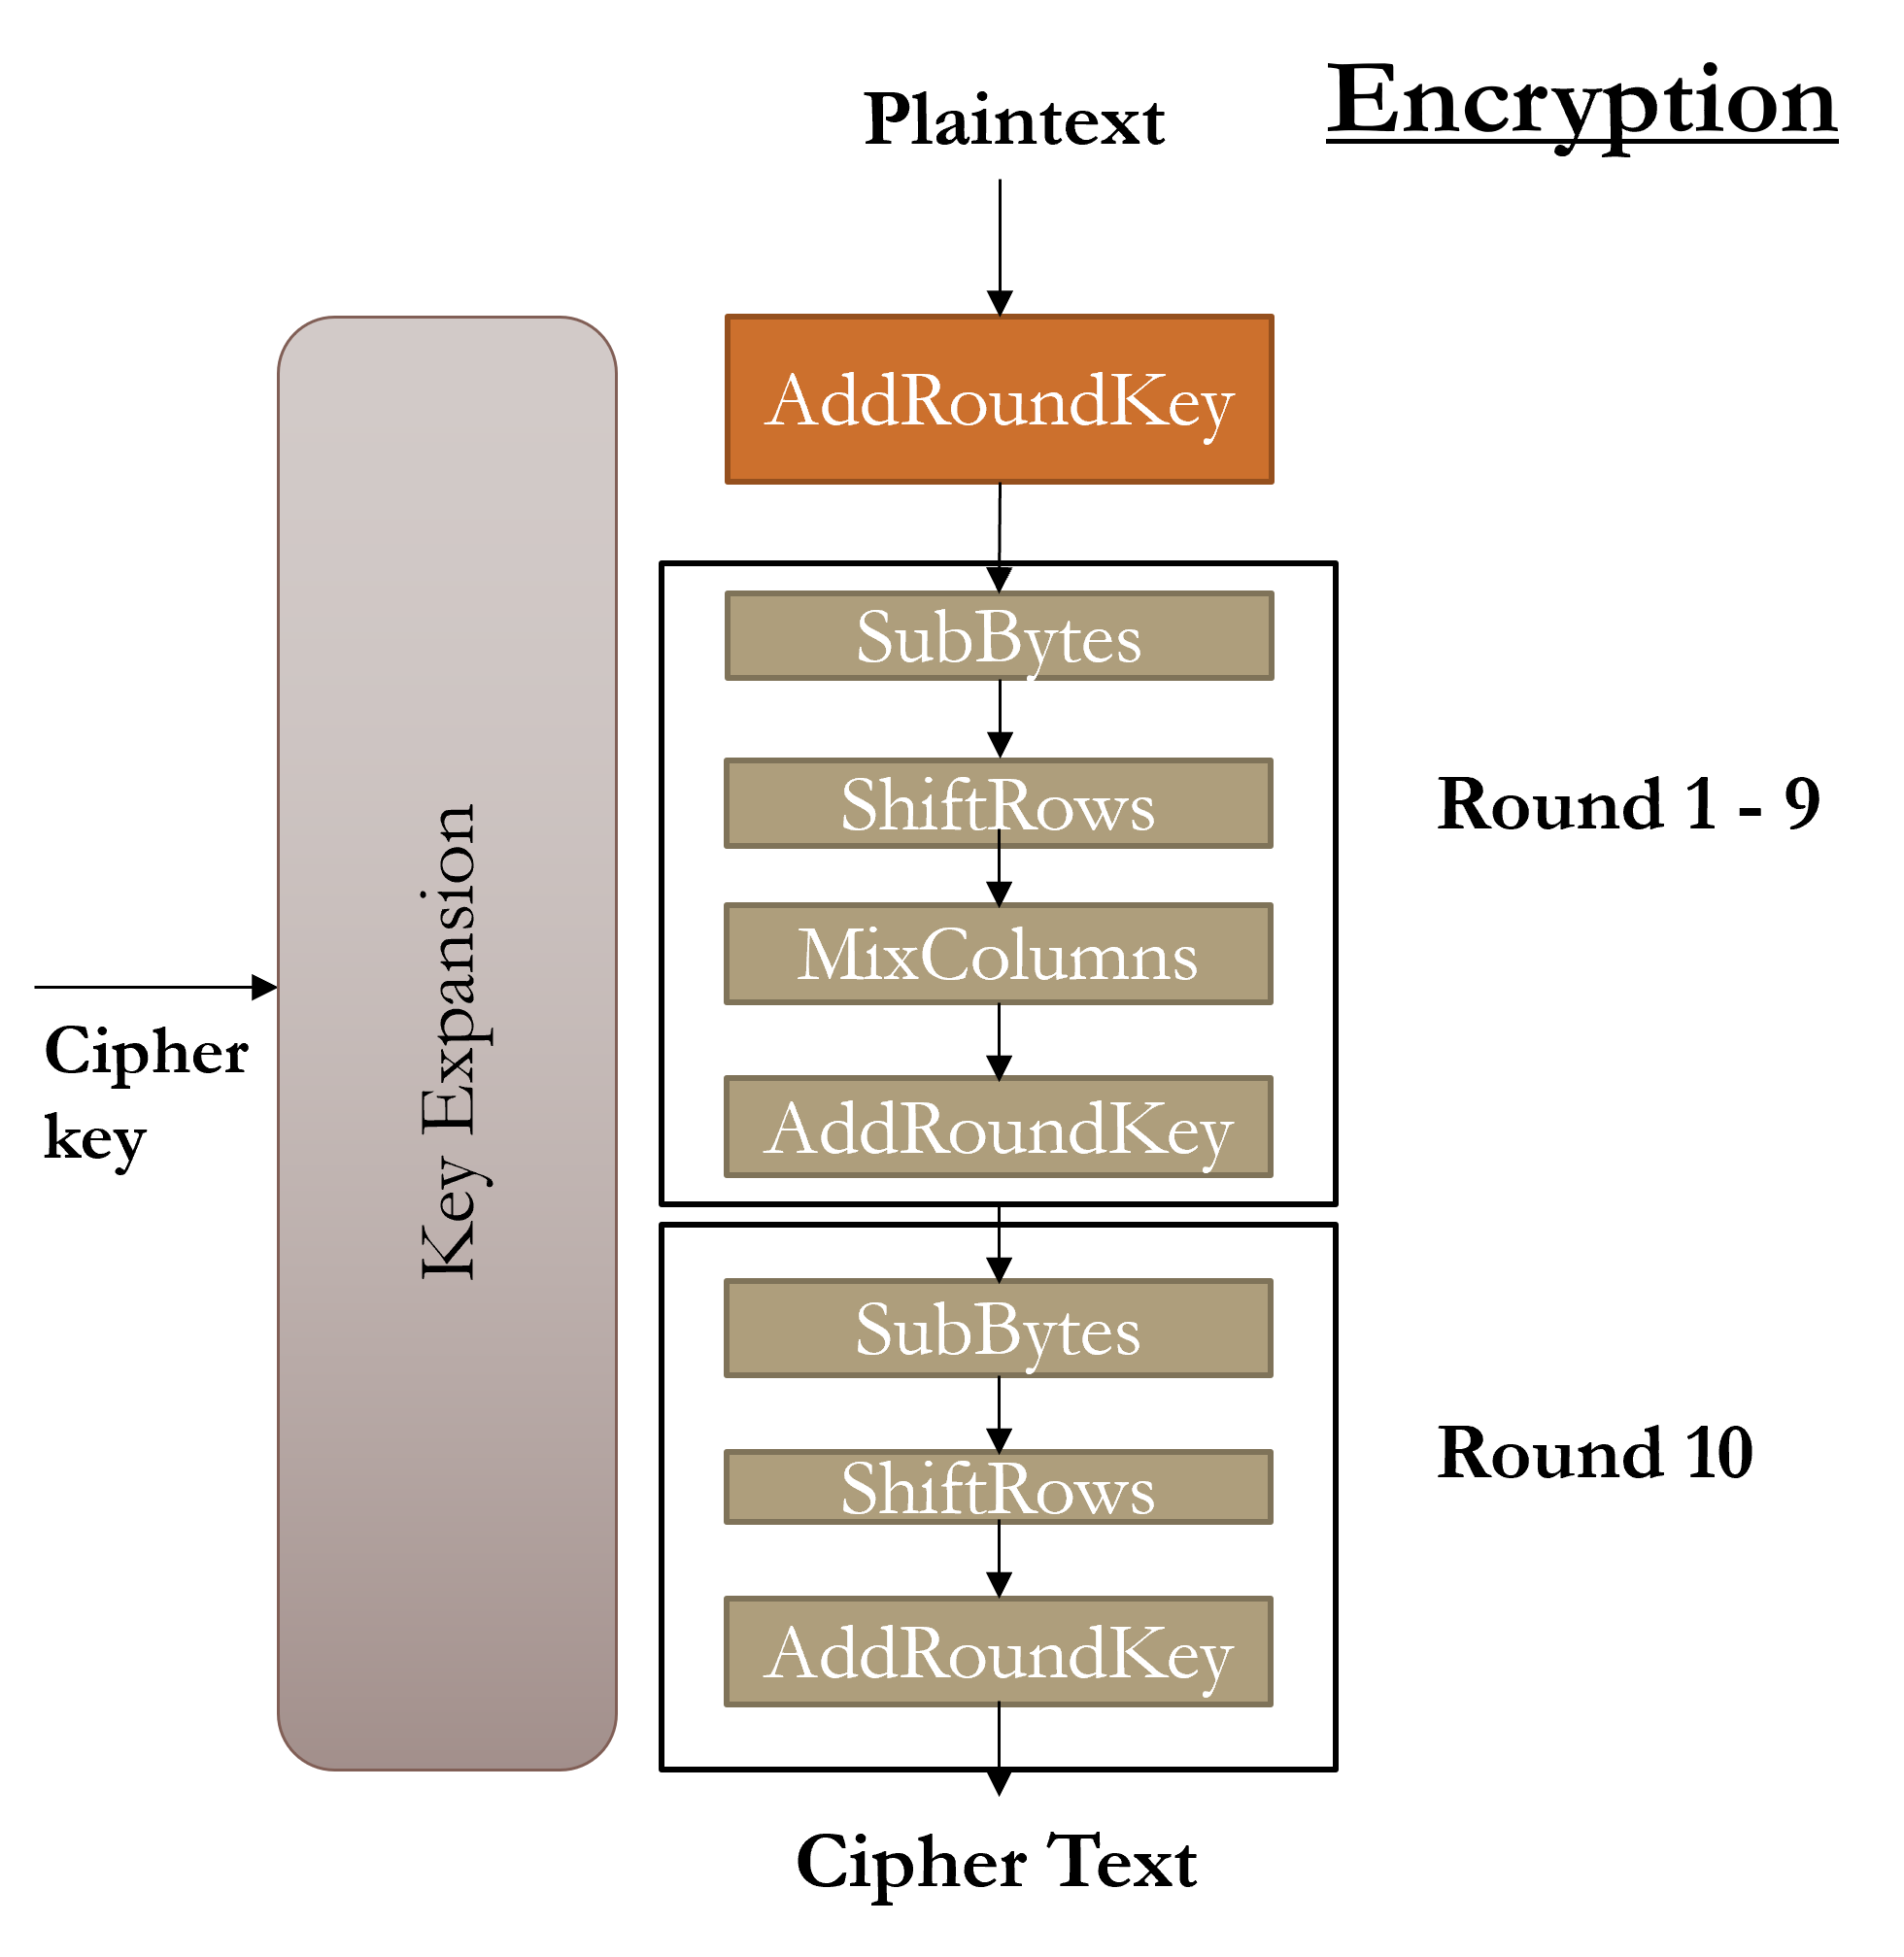
\includegraphics[width=\textwidth]{aes_encryption.png}
				\caption{AES Encryption Algorithm}
			\end{figure}
		\end{column}

		\pause

		\begin{column}{0.45\textwidth} % Left column width
			\begin{figure}
				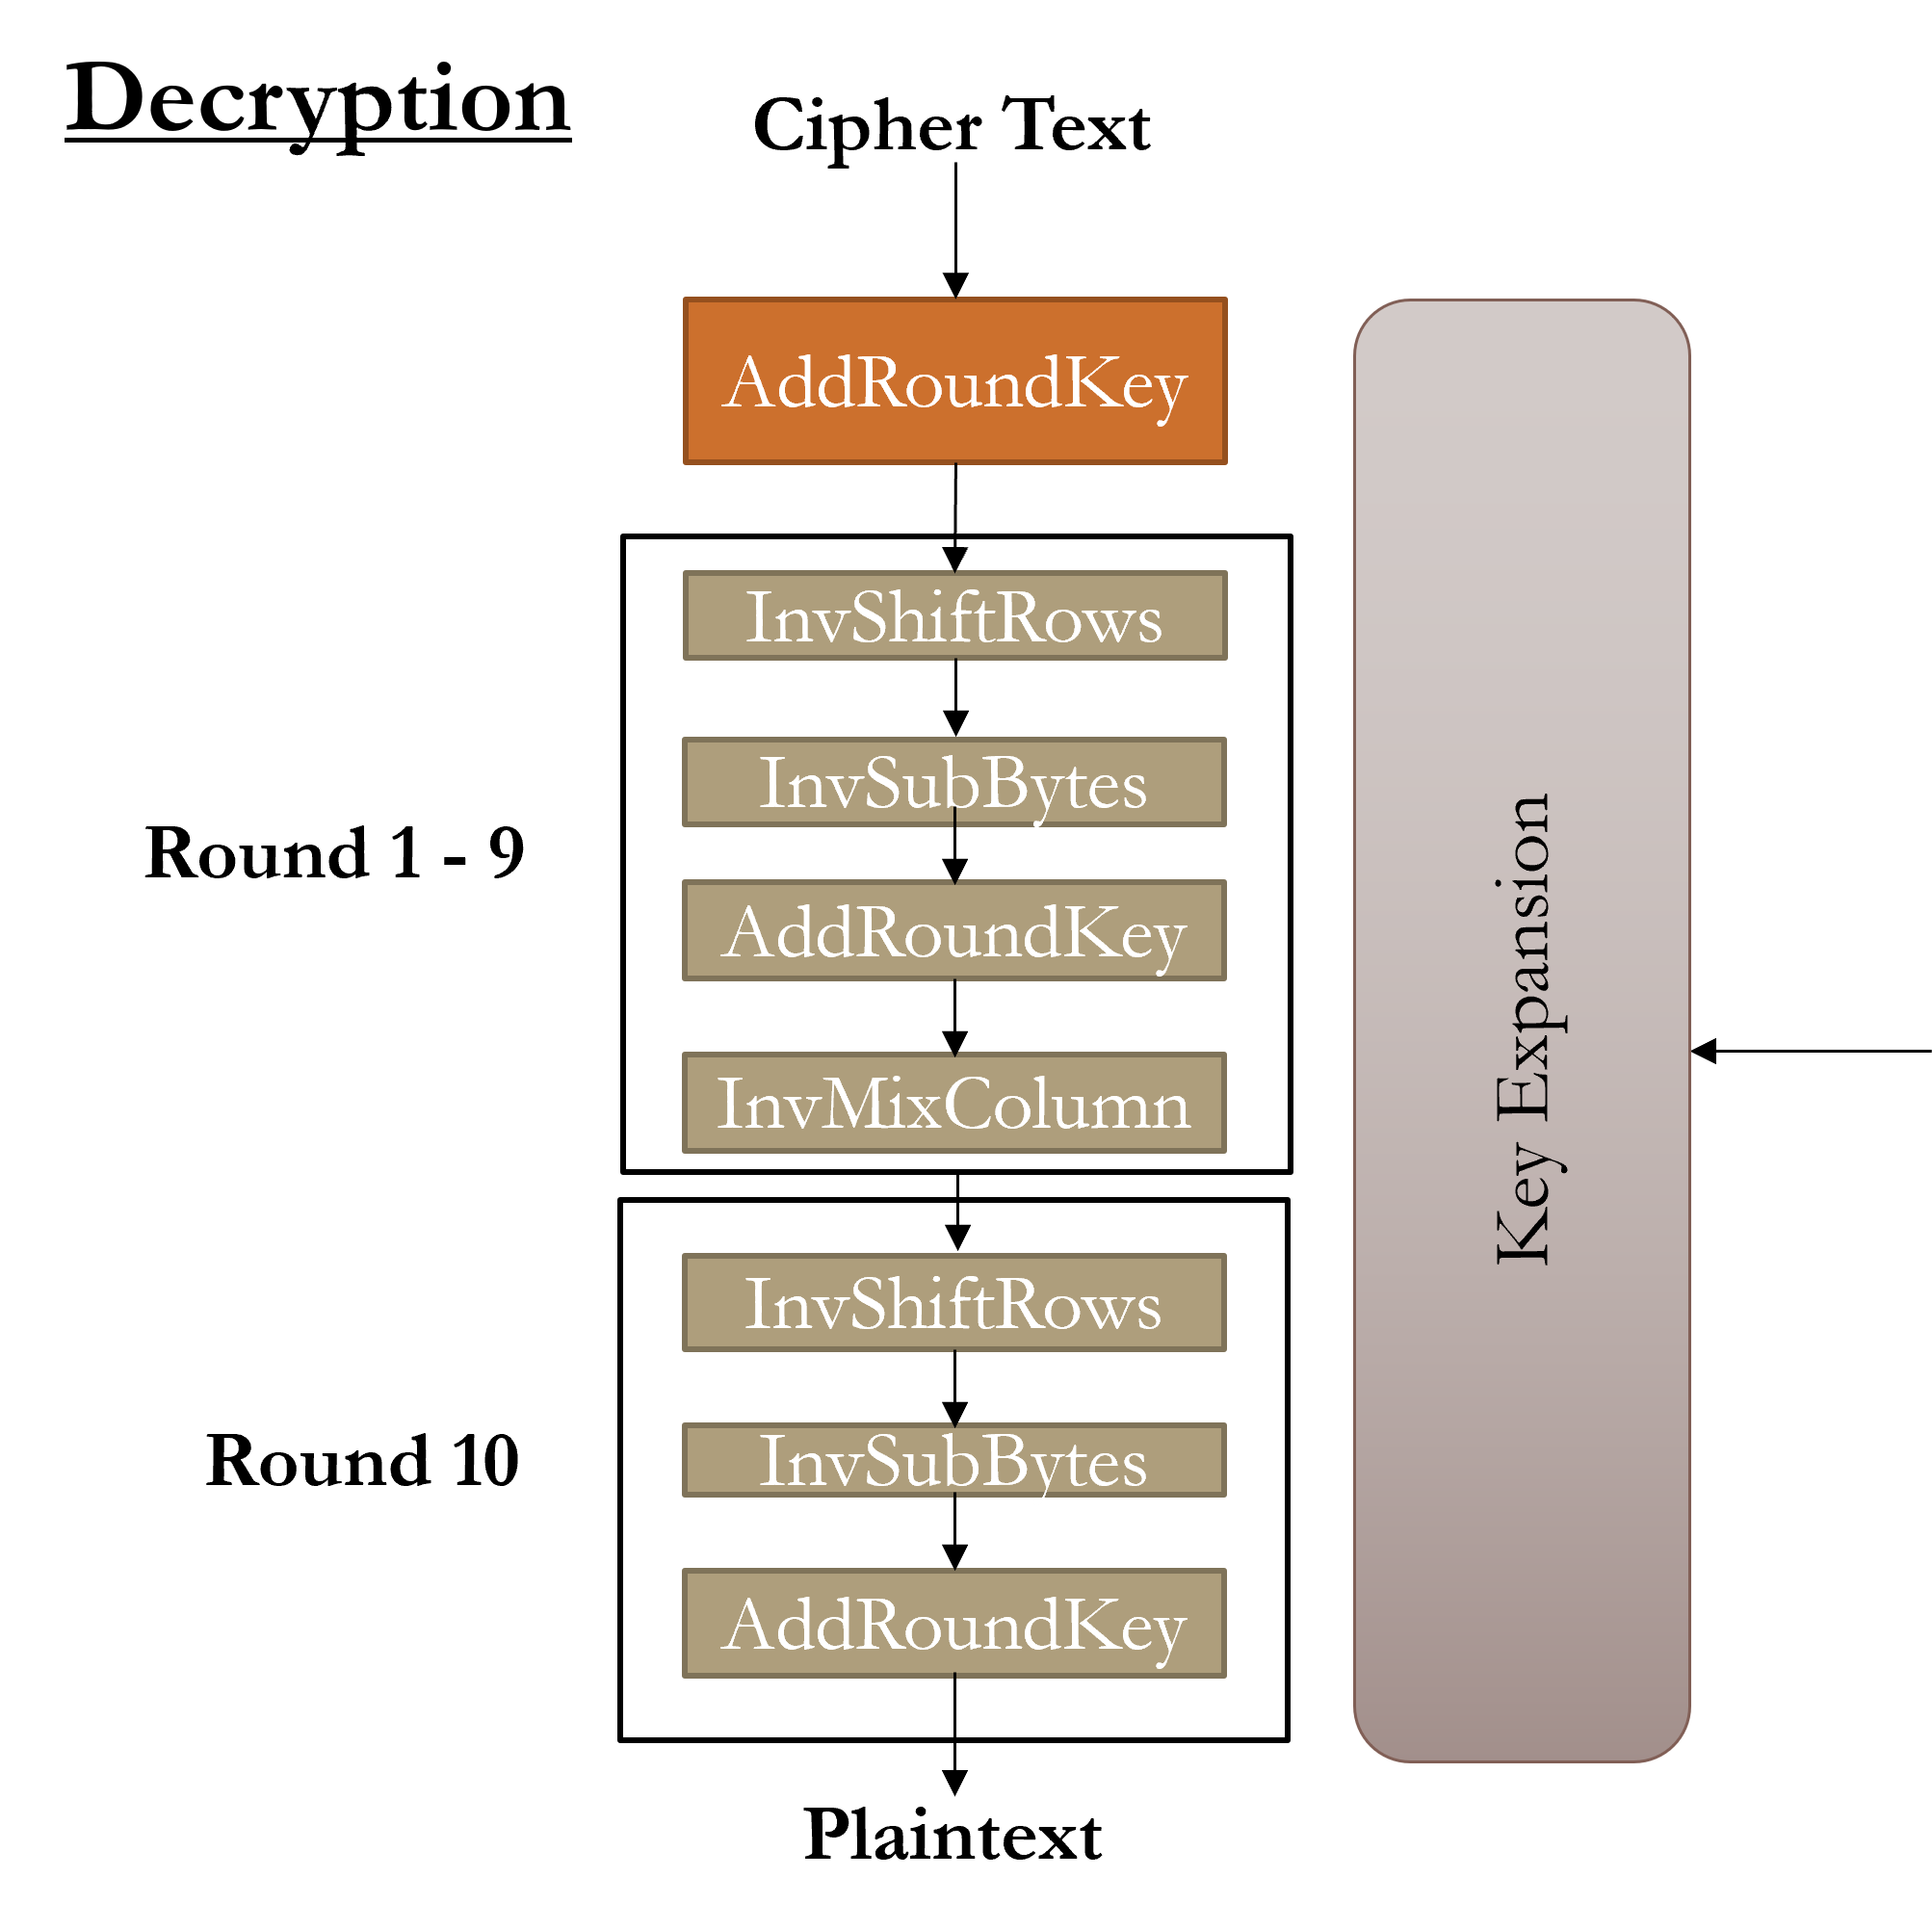
\includegraphics[width=\textwidth]{aes_decryption.png}
				\caption{AES Decryption Algorithm}
			\end{figure}
		\end{column}
	\end{columns}
\end{frame}

\begin{frame}
	\frametitle{Previous Side Project: MIPS Implementation}
	\begin{figure}
		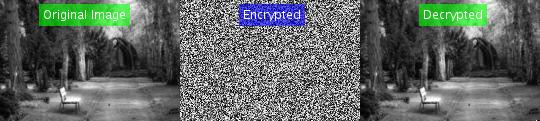
\includegraphics[width=\textwidth]{182_coe301_side_project.jpg}
		\caption{AES MIPS Implementation and Example}
	\end{figure}
\end{frame}


\section{Assembly Template}
\begin{frame}
	\frametitle{MIPS Assembly Language Program Template}
	
	\begin{columns}[c] % The "c" option specifies centered vertical alignment while the "t" option is used for top vertical alignment
		
		\begin{column}{0.5\textwidth} % right column width
			\begin{figure}
				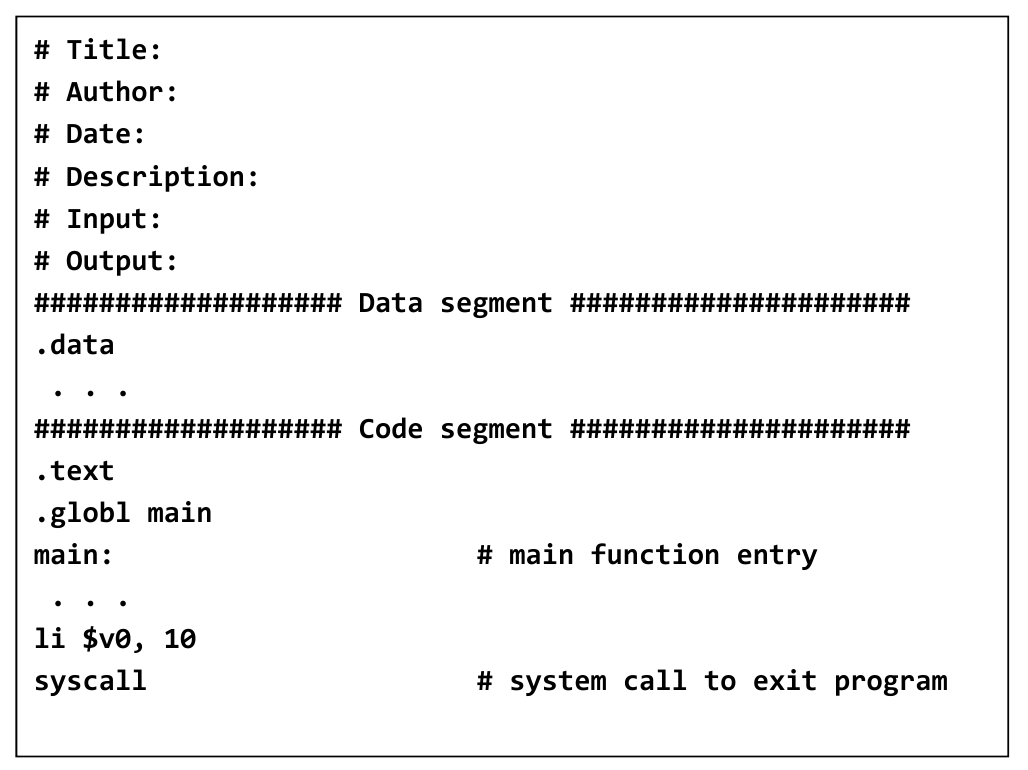
\includegraphics[width=0.9\linewidth]{mips_assembly_program_language.png}
				\caption{MIPS Assembly Program Language}
			\end{figure}
		\end{column}


		\begin{column}{0.5\textwidth} % Left column width
			\begin{itemize}
				\item Comments start with '\#' 
				\item Directives start with '.'
				\item Instructions are usually written in lower case; however, you can write them in uppercase as well.
				\item Registers name or number starts with '\$'.
			\end{itemize}
		\end{column}
	\end{columns}
\end{frame}

%------------------------------------------------

% \section{Programming Cycle}
\begin{frame}
	\frametitle{Edit-Assemble-Link-Run Cycle}
	\begin{figure}
		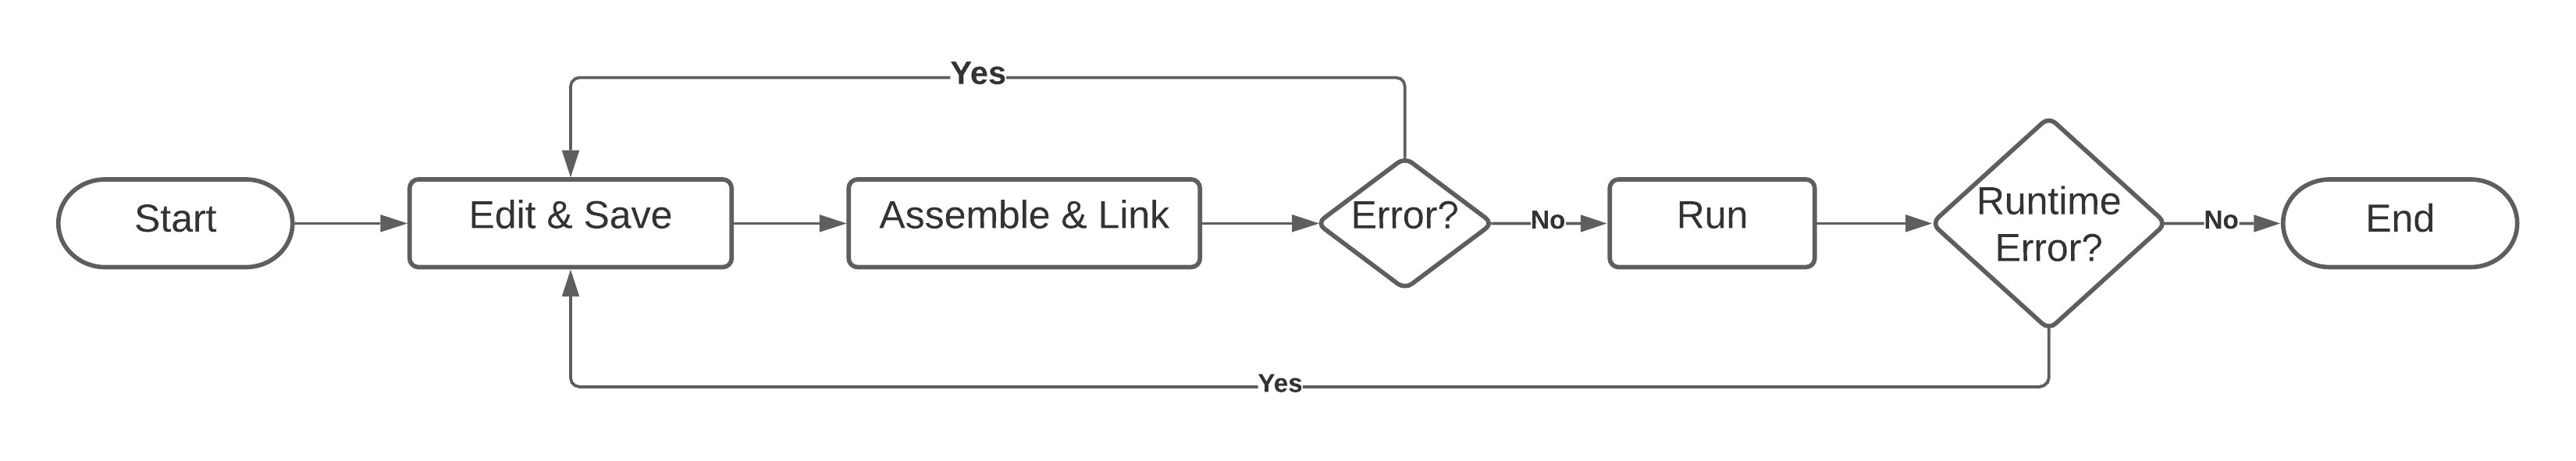
\includegraphics[width=\linewidth]{program_cycle.png}
	\end{figure}
\end{frame}

\section{MIPS Instr. Formats}
\begin{frame}
	\frametitle{MIPS Instr. Formats}
	\begin{columns}[c] % The "c" option specifies centered vertical alignment while the "t" option is used for top vertical alignment
		\begin{column}{0.44\textwidth} % Left column width
			\begin{itemize}
					\item R-Type Format
					\begin{itemize}
						\item Requires two register operands
						\item e.g. add \$t0, \$t1, \$t2
					\end{itemize}
				\visible<2->{
					\item I-Type Format
					\begin{itemize}
						\item Requires two operands: a register and 16-bit immediate value
						\item e.g. addi \$t0, \$t1, 301
					\end{itemize}
				}
				\visible<3->{
					\item J-Type Format 
					\begin{itemize}
						\item Used for jump instructions with 26-bit immediate value
						\item e.g. j loop						
				  	\end{itemize}
				}
			\end{itemize}
		\end{column}
	
		\begin{column}{0.56\textwidth} % right column width
			\visible<1->{
				\begin{table}
					\begin{tabular}{|p{0.11\textwidth}|p{0.0875\textwidth}|p{0.0875\textwidth}|p{0.0875\textwidth}|p{0.0875\textwidth}|p{0.11\textwidth}|}
						\toprule
						\textbf{$ op^6 $} & \textbf{$ rs^5 $} & \textbf{$ rt^5 $} & \textbf{$ rd^5 $} & \textbf{$ sa^5 $} & \textbf{$ func^6 $} \\
						\bottomrule
					\end{tabular}
					\caption{R-Type Instruction Format}
				\end{table}
			}
			\visible<2->{
				\begin{table}
					\begin{tabular}{|p{0.105\textwidth}|p{0.0875\textwidth}|p{0.0875\textwidth}|p{0.4\textwidth}|}
						\toprule
						\textbf{$ op^6 $} & \textbf{$ rs^5 $} & \textbf{$ rt^5 $} & \textbf{$ immediate^{16} $} \\
						\bottomrule
					\end{tabular}
					\caption{I-Type Instruction Format}
				\end{table}
			}
			\visible<3->{
				\begin{table}
					\begin{tabular}{|p{0.105\textwidth}|p{0.7\textwidth}|}
						\toprule
						\textbf{$ op^6 $} & \textbf{$ immediate^{26} $} \\
						\bottomrule
					\end{tabular}
					\caption{J-Type Instruction Format}
				\end{table}
			}
		\end{column}
	\end{columns}
\end{frame}

%------------------------------------------------

\section{MIPS Registers \& System Calls}
\begin{frame}
	\frametitle{MIPS General Purpose Registers}
	
	\begin{table}
		\centering
		% \caption{MIPS General Purpose Registers}
		\resizebox{\linewidth}{!}{%
			\begin{tabular}{|l|l|l|}
				\toprule
				\textbf{Register Name} & \textbf{Register No.} & \textbf{Register Usage} \\
				\midrule
				\$zero        & \$0            & Always zero, forced by hardware                             \\ \hline
				\rowcolor{orange} \$at          & \$1            & Assembler Temporary register, reserved for assembler use    \\ \hline
				\$v0 - \$v1   & \$2  - \$3     & Results of a function                                       \\ \hline
				\$a0 - \$a3   & \$4  - \$7     & Arguments of a function                                     \\ \hline
				\$t0 - \$t7   & \$8  - \$15    & Registers for storing temporary values                      \\ \hline
				\$s0 - \$s7   & \$16 - \$23    & Registers that should be saved across function calls        \\ \hline
				\$t8 - \$t9   & \$24 - \$25    & Registers for storing more temporary values                 \\ \hline
				\rowcolor{orange} \$k0 - \$k1   & \$26 - \$27    & Registers reserved for the OS kernel use                    \\ \hline
				\rowcolor{orange} \$gp          & \$28           & Global Pointer register that points to global data          \\ \hline
				\rowcolor{orange} \$sp          & \$29           & Stack Pointer register that points to top of stack          \\ \hline
				\rowcolor{orange} \$fp          & \$30           & Frame Pointer register that points to stack frame           \\ \hline
				\rowcolor{orange} \$ra          & \$31           & Return Address register used to return from a function call \\
				\bottomrule
			\end{tabular}%
		}
	\end{table}
\end{frame}

% \section{System Calls}

\begin{frame}
	\frametitle{System Calls}
	System calls provide system services, mainly for input and output, are available for use by your MIPS program. 
	\begin{table}
		\caption{Partial List of System Calls}
		\centering
		\resizebox{\textwidth}{!}{%
			\begin{tabular}{|l|c|l|l|}
				\toprule
				\textbf{Service} 	& \textbf{code in \$v0}    & \textbf{Arguments} 															                              & \textbf{Results} 	  \\
				\midrule
				Print Integer   	& 1  					   & \$a0 = integer to print 														                              &                       \\ \hline
				Print String    	& 4  					   & \$a0 = address of null-terminated string 										                              &                       \\ \hline
				Read Integer    	& 5  					   &  																				                              & \$v0 = integer read   \\ \hline
				Read String     	& 8  					   & \begin{tabular}[l]{@{}l@{}}\$a0 = address of input buffer\\ \$a1 = maximum number of characters\end{tabular} & 					  \\ \hline
				Exit Program    	& 10 					   & 																				                              & Terminate Program	  \\ \hline
				Print Character 	& 11 					   & \$a0 = character to print 													                                  &                       \\ \hline
				Read Character  	& 12 					   &  																				                              & 					  \\
				\bottomrule
			\end{tabular}%
		}
	\end{table}
\end{frame}


%------------------------------------------------

\section{Live Examples}

\begin{frame}
	\frametitle{Live Examples}
	
\end{frame}

%------------------------------------------------

\section{Tasks}

\begin{frame}
	\frametitle{Task \#1}
	Write a MIPS program where you ask the user to enter 3 integers \textbf{a}, \textbf{b}, and \textbf{c}. Then, calculate and print the value of \textbf{z} based on the following equation. 
	\begin{equation*}
		z = (6a - 4b) - (3c - 20)
	\end{equation*}
	\centering
	Sample Run


	\minibox[frame,pad=8pt]{
		\color{black} Enter a: \color{blue} 4 \\
		\color{black} Enter b: \color{blue} 6 \\ 
		\color{black} Enter c: \color{blue} 2 \\ 
		\color{black} z = \color{darkGreen} 14 \\
	}		
\end{frame}

\begin{frame}
	\frametitle{Task \#2}
	Write a MIPS program where you prompt the user for his \textbf{name}. Then, print the following message

	\centering
	\textquotedblleft Welcome to COE301, $<$name$>$ \textquotedblright

	\begin{flushleft}
		Assume the maximum length for a name is 20 characters.
	\end{flushleft}
	

	\centering
	Sample Run


	\minibox[frame,pad=4pt]{
	 	\color{black} Enter your name: \color{blue} Khalid \\ 
	 	\color{black} Welcome to COE301, \color{darkGreen} Khalid
	}	
\end{frame}

%----------------------------------------------------------------------------------------

\end{document} 
